% Technical documentation of the RAG on Medical Documents project.
% Build from this folder: pdflatex main.tex (twice, for the table of contents).
% The result tables are read from ../report/generated/ and the plots from ../../results/;
% when a file is missing, a red TODO is printed instead.
\documentclass[10pt,a4paper]{article}

\usepackage[T1]{fontenc}
\usepackage[utf8]{inputenc}
\usepackage{lmodern}
\usepackage{microtype}
\usepackage[a4paper,margin=2cm,headheight=14pt]{geometry}
\usepackage{graphicx}
\usepackage{booktabs}
\usepackage{tabularx}
\usepackage{array}
\usepackage{amsmath}
\usepackage{xcolor}
\usepackage{enumitem}
\usepackage{fancyhdr}
\usepackage{caption}
\usepackage{float}
\usepackage{listings}
\usepackage{pgfplots}
\pgfplotsset{compat=1.18}
\usepackage{xurl}
\usepackage[hidelinks]{hyperref}

% Anything not yet known is printed in red, so that it cannot be missed.
\newcommand{\TODO}[1]{\textcolor{red}{\textbf{[TODO: #1]}}}
% Code names (file names, functions, constants) in typewriter, underscores kept as typed.
\newcommand{\code}[1]{\texttt{\detokenize{#1}}}
% Paths to the generated tables and to the result files, relative to this folder.
\newcommand{\gen}{../report/generated}
\newcommand{\res}{../../results}

\lstset{basicstyle=\ttfamily\small, breaklines=true, columns=fullflexible,
        frame=single, rulecolor=\color{black!25}, backgroundcolor=\color{black!3},
        xleftmargin=0.5em, xrightmargin=0.5em, aboveskip=0.6em, belowskip=0.6em}
\setlist{itemsep=0.15em, topsep=0.3em}
\setlength{\parskip}{0.2em}
\setlength{\parindent}{0pt}
\captionsetup{font=small, labelfont=bf, justification=raggedright, singlelinecheck=true}
\renewcommand{\arraystretch}{1.15}

\pagestyle{fancy}
\fancyhf{}
\fancyhead[L]{\small \TODO{school name}}
\fancyhead[R]{\small Group \TODO{NN} -- RAG on Medical Documents}
\fancyfoot[C]{\small \thepage}

\begin{document}

\begin{center}
  {\LARGE\bfseries RAG on Medical Documents}\\[0.4em]
  {\Large Technical documentation}\\[0.8em]
  Boussoualim Yassine \quad Benahcene Mohamed Wassim \quad Aissaoui Anes Safouane \quad Djerdali Mohamed Achraf\\[0.3em]
  Group \TODO{group number} \quad -- \quad \TODO{school header}\\
  LLM Final Projects 2026-2027, Prof.\ A.\ Moussaoui, Project 2\\[0.3em]
  {\small Describes the code of branch \code{eval-prep} at commit \code{98ad7c7} (15 November 2026).}
\end{center}

\noindent\textbf{In short.} The system answers medical questions from 20 WHO guidelines and 30 open-access
PubMed Central articles. It retrieves five passages, asks a free language model on OpenRouter to answer
only from them and to cite them by number, and keeps the answer only if the citations point at the
given passages. When a cross-encoder judges that no passage answers the question, or the model does
not cite the passages, the system replies with one fixed sentence:
``I cannot answer this question from the provided documents.''
It is a student project. It is not medical advice.



\section{Architecture and data flow}
\label{sec:architecture}

Figure~\ref{fig:architecture} shows the system as the code builds it. It has three parts. The first
runs once and builds the index. The second runs for every question, in the web app or on the
command line. The third measures the second on a fixed question set. The source of the figure is
\code{docs/technical/architecture.dot}; \code{dot -Tpng -Gdpi=200} renders it to
\code{architecture_diagram.png}.

\begin{figure}[p]
  \centering
  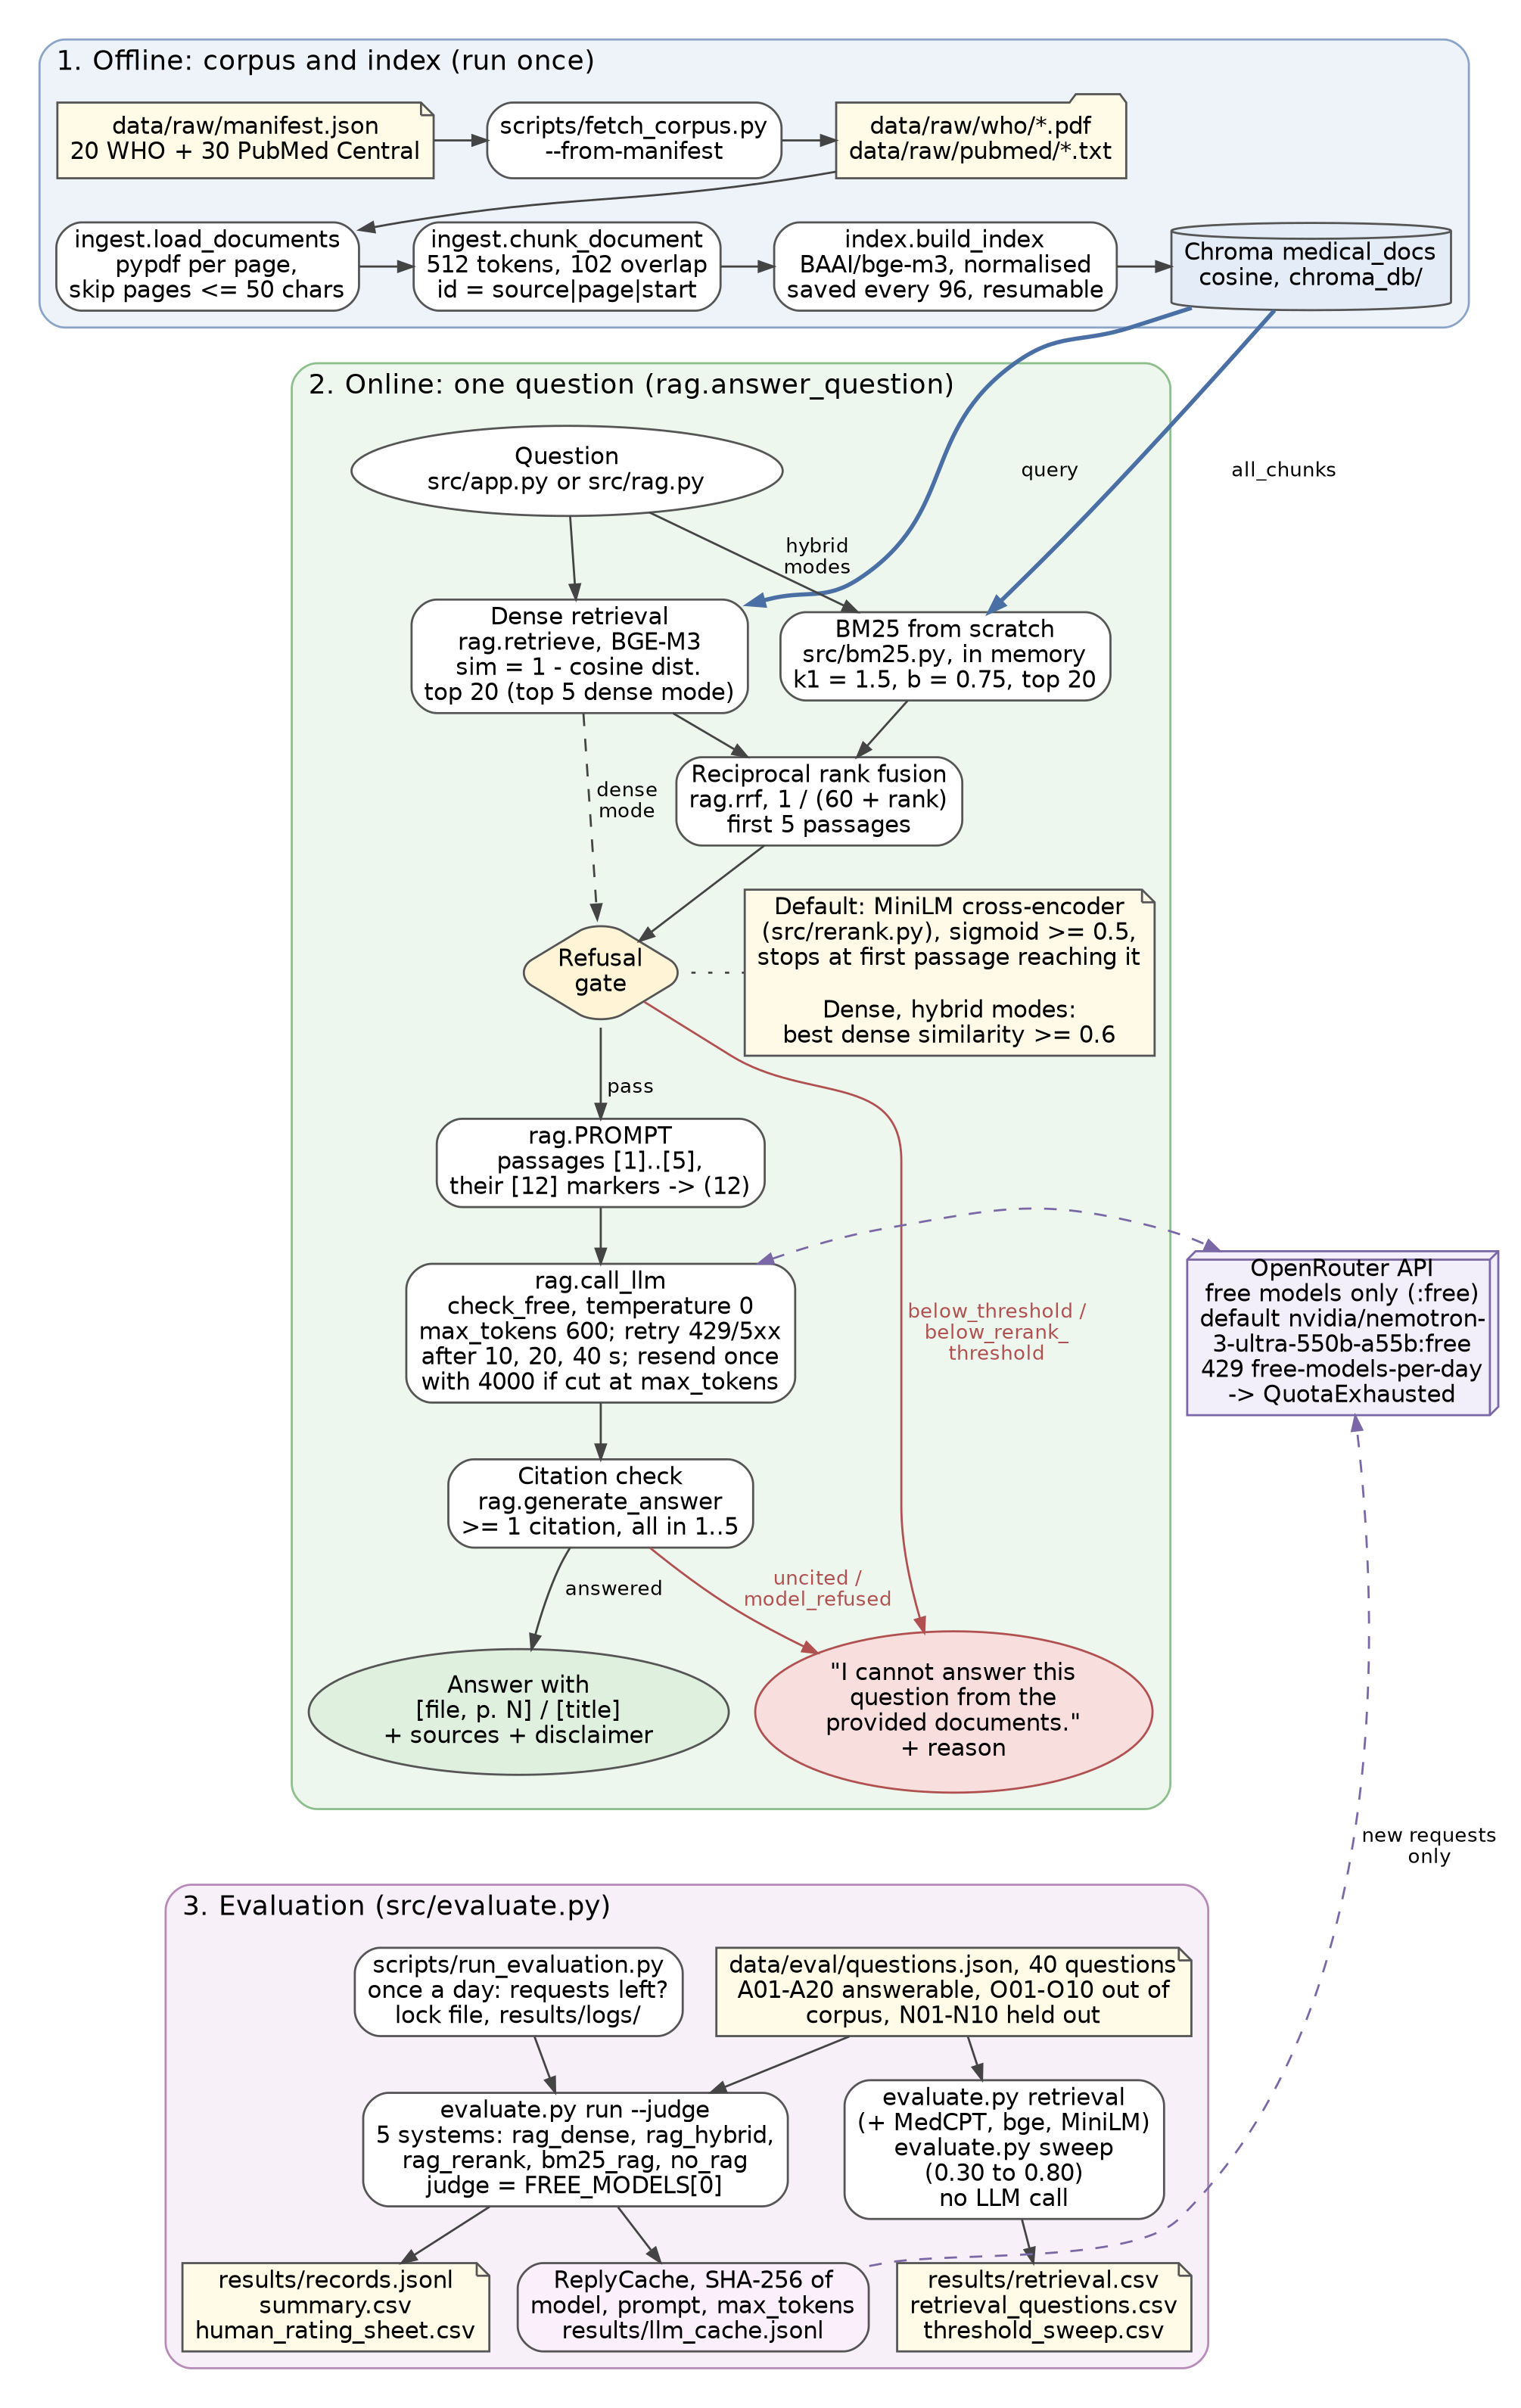
\includegraphics[height=0.9\textheight,width=\textwidth,keepaspectratio]{architecture_diagram.png}
  \caption{Architecture as built. Blue: offline indexing. Green: the path of one question, with
  its two refusal exits in red. Purple: the evaluation, which calls the same functions and sends
  every model request through a reply cache. Dashed purple arrows are network calls to OpenRouter.}
  \label{fig:architecture}
\end{figure}

\subsection{Offline: from documents to an index}

\begin{enumerate}[leftmargin=1.5em]
  \item The script \code{scripts/fetch_corpus.py}, run with \code{--from-manifest}, downloads the
        50 documents of the manifest (\nolinkurl{data/raw/manifest.json}): 20 WHO guidelines as PDF
        files from WHO IRIS, and 30 PubMed Central articles as plain text from the Europe PMC
        full-text API.
  \item \code{ingest.load_documents} reads each WHO PDF page by page with pypdf and skips pages of
        50 characters or fewer. Each PubMed article becomes one record with no page, cited by its
        title from the manifest.
  \item \code{ingest.chunk_document} cuts each record into windows of 512 tokens of the BGE-M3
        tokenizer, with 102 tokens of overlap, so a window moves by 410 tokens. A chunk keeps its
        source, page and kind. Its id is \code{source|page|start_token}.
  \item \code{index.build_index} embeds the chunks with \code{BAAI/bge-m3} (normalised vectors) and
        stores them in the persistent Chroma collection \code{medical_docs}, created with cosine
        distance. It saves every 96 chunks and, on a restart, only embeds the ids that are missing.
\end{enumerate}

\subsection{Online: one question}

\code{rag.answer_question} runs the whole path. The app offers three modes and the command line
has the same three (\code{--hybrid}, \code{--rerank}).

\begin{enumerate}[leftmargin=1.5em]
  \item \textbf{Retrieval.} The question is embedded with BGE-M3 and Chroma returns the nearest
        chunks; similarity is $1 - \text{cosine distance}$. In \emph{dense} mode the 5 nearest
        chunks are the passages. In the two hybrid modes, the 20 nearest chunks and the 20 best
        BM25 chunks are fused by reciprocal rank fusion and the first 5 are the passages. BM25 is
        built in memory at start-up from every chunk stored in Chroma, so both retrievers see the
        same chunks.
  \item \textbf{Refusal gate.} In \emph{dense} and \emph{hybrid} modes, the question is refused when
        the best dense similarity is below 0.6 (\code{SIM_THRESHOLD}). In the default mode,
        \emph{hybrid + cross-encoder gate}, the MiniLM cross-encoder scores the question with each
        passage, in retrieval order, and the question is refused when no passage reaches 0.5
        (\code{RERANK_THRESHOLD}) after a sigmoid. A refused question never reaches the model.
  \item \textbf{Generation.} The passages are numbered \code{[1]} to \code{[5]} under their source
        label, and the prompt asks a free model on OpenRouter to answer only from them, to cite a
        number after each claim, and to say the refusal sentence if the passages do not hold the
        answer. Reference markers inside the passages, such as \code{[12]}, are shown to the model
        as \code{(12)}.
  \item \textbf{Citation check.} The reply is kept only if it cites at least one passage and every
        cited number is between 1 and the number of passages. Each number is then replaced by a
        readable label, \code{[file, p. N]} for a WHO page or \code{[article title]} for a PubMed
        article. Otherwise, or if the model wrote the refusal sentence itself, the answer is the
        refusal sentence.
\end{enumerate}

Every result carries a reason, shown in the app under a refusal (Table~\ref{tab:reasons}).

\begin{table}[H]
  \centering\small
  \begin{tabularx}{\textwidth}{@{}l l X@{}}
    \toprule
    Reason & Set by & Meaning \\
    \midrule
    \code{answered} & \code{generate_answer} & Cited answer, every citation is a given passage. \\
    \code{below_threshold} & \code{answer_question} & Best dense similarity below the threshold; model not called. \\
    \code{below_rerank_threshold} & \code{answer_question} & No passage reaches the cross-encoder threshold; model not called. \\
    \code{uncited} & \code{generate_answer} & No citation, or a number outside 1..5. \\
    \code{model_refused} & \code{generate_answer} & The model wrote the refusal sentence. \\
    \code{no_context} & \code{generate_answer} & No passage was retrieved. \\
    \bottomrule
  \end{tabularx}
  \caption{The six reasons a result can carry.}
  \label{tab:reasons}
\end{table}

\subsection{Evaluation}

\code{src/evaluate.py} has three commands. \code{retrieval} and \code{sweep} make no model call:
they compare the retrievers and the gates on the question set and calibrate the similarity
threshold. \code{run} answers the question set with five systems (Section~\ref{sec:results}) and
writes one record per answer. It wraps \code{rag.call_llm} in a \code{ReplyCache}, so an identical
request (same model, prompt and token budget) is sent once and later reused.
\code{scripts/run_evaluation.py} runs one day's share of \code{run}, because the account allows 50
free-model requests a day.

\section{Components}
\label{sec:components}

The code is seven Python files in \code{src/} and four scripts in \code{scripts/}
(Table~\ref{tab:files}). Every function and class has a docstring. The dependencies are pinned in
\code{requirements.txt}: PyTorch 2.15.0 (CPU build), sentence-transformers 6.3.0, chromadb 1.5.9,
pypdf 7.1.0, cryptography 50.0.2, gradio 6.32.0 and pytest 9.2.0. The OpenRouter call uses only
the standard library (\code{urllib}).

\begin{table}[H]
  \centering\small
  \begin{tabularx}{\textwidth}{@{}l X >{\raggedright\arraybackslash}p{4.6cm}@{}}
    \toprule
    File & Role & Key constants \\
    \midrule
    \code{src/ingest.py} & Reads the PDFs and text files, cuts them into chunks with stable ids. & \code{CHUNK_TOKENS} 512, \code{OVERLAP_TOKENS} 102 \\
    \code{src/index.py} & Embeds the chunks into Chroma (resumable), opens the index, reads every chunk back. & \code{EMBED_MODEL}, \code{COLLECTION} \\
    \code{src/bm25.py} & Okapi BM25 over the chunks, written from scratch with the standard library. & \code{k1} 1.5, \code{b} 0.75 \\
    \code{src/rag.py} & Retrieval, fusion, both gates, prompt, OpenRouter call, citation check, command line. & \code{TOP_K} 5, \code{CANDIDATES} 20, \code{SIM_THRESHOLD} 0.6, \code{RERANK_THRESHOLD} 0.5 \\
    \code{src/rerank.py} & Cross-encoder scoring: the gate score and reordering. & \code{GATE_RERANKER} \code{minilm} \\
    \code{src/app.py} & Gradio page: question, model, mode, threshold, answer, sources table. & \code{DISCLAIMER}, \code{MODES} \\
    \code{src/evaluate.py} & Retrieval comparison, threshold sweep, evaluation of five systems. & \code{THRESHOLDS}, \code{JUDGE_MAX_TOKENS} 4000 \\
    \midrule
    \code{scripts/fetch_corpus.py} & Downloads the corpus, from the manifest or by topic search. & 15 MB cap per PDF \\
    \code{scripts/make_dataset_links.py} & Writes \code{docs/dataset_links.md} from the manifest. & \\
    \code{scripts/check_eval_set.py} & Checks that the 20 evidence quotes are on their recorded page. & \\
    \code{scripts/run_evaluation.py} & Runs one day's share of the evaluation, with a lock and a log. & \code{STEPS} \\
    \bottomrule
  \end{tabularx}
  \caption{Files of the project and their role.}
  \label{tab:files}
\end{table}

\paragraph{Ingestion and index (\code{ingest.py}, \code{index.py}).}
The chunker receives the tokenizer as an argument. In production it is the tokenizer of BGE-M3,
so a window is exactly 512 tokens of the embedding model; the tests pass a fake tokenizer with one
token per word. The chunk id \code{source|page|start_token} is the same on every run for the same
settings, which is what makes the build resumable: the chunks still to embed are the set difference
between the corpus ids and the ids Chroma already holds, and stored ids that no longer match a chunk
are deleted. A PubMed chunk has no page; it is stored as $-1$ in Chroma and read back as none.

\paragraph{BM25 (\code{bm25.py}).}
An inverted index maps each term to the chunks that contain it and how often. Tokens are runs of
lowercase letters and digits. The score is Okapi BM25 with $k_1 = 1.5$ and $b = 0.75$, and an idf
with 1 inside the logarithm, $\ln\bigl(1 + (N - n + 0.5)/(n + 0.5)\bigr)$, which stays positive for
a term found in more than half the chunks (the Lucene variant). The code follows two
build-your-own-x tutorials and Robertson and Zaragoza (2009); its docstring credits them.

\paragraph{Retrieval and generation (\code{rag.py}).}
\code{rrf} gives a chunk at rank $r$ (counted from 1) a score of $1/(60 + r)$ per list and sorts by
the sum, after Cormack, Clarke and Buettcher (SIGIR 2009). \code{call_llm} sends one chat request
with \code{temperature} 0 and \code{max_tokens} 600. Its first statement is \code{check_free}, which
raises unless the model id ends in \code{:free} or is \code{openrouter/free}. \code{load_context}
loads the key, the index, BGE-M3, BM25 and the gate cross-encoder, and exits with one line when the
key or the index is missing.

\paragraph{Cross-encoder (\code{rerank.py}).}
\code{gate_score} applies a sigmoid to the cross-encoder's raw score (a logit), so 0.5 is the
model's own boundary between relevant and not relevant. It scores the passages one at a time and,
with \code{stop_at}, stops at the first one that reaches it. \code{rerank} sorts hits by score; it
is used only by the retrieval comparison. Three models are registered: \code{minilm}
(\code{cross-encoder/ms-marco-MiniLM-L6-v2}, the gate), \code{medcpt}
(\code{ncbi/MedCPT-Cross-Encoder}) and \code{bge} (\code{BAAI/bge-reranker-v2-m3}).

\paragraph{App (\code{app.py}).}
A Gradio page on \url{http://127.0.0.1:7860} with a question box, a model menu limited to the five
free models of \code{FREE_MODELS}, a choice of mode (default: hybrid + cross-encoder gate), a
threshold slider from 0 to 1 that applies to the gate of the chosen mode, the answer with the
disclaimer, and a table of the five passages with their page, similarity and whether they were
cited. Changing the mode resets the slider to that gate's default (0.6 or 0.5). An empty question
and a failed model call become a message instead of a crash.

\paragraph{Evaluation (\code{evaluate.py}, \code{run_evaluation.py}).}
\code{run} is resumable: each answer is appended to \nolinkurl{results/records.jsonl} with the threshold
it was made with, and a rerun skips what is there. It refuses to mix records made at another
threshold. \code{run_evaluation.py} asks OpenRouter how many free requests are left today (the
question itself uses none), runs the five systems with the default model and then
\code{rag_rerank} with the second free model, each with \code{--judge}, and appends its output to
\code{results/logs/<UTC date>.log}.

\section{Technical choices}
\label{sec:choices}

Each choice below gives the reason and, where we have one, the measurement behind it. Unless said
otherwise, the retrieval figures come from \code{results/retrieval.csv} and
\code{results/retrieval_questions.csv}, written by \code{evaluate.py retrieval} on the original 30
questions (20 answerable, 10 out of corpus) before the 10 held-out questions existed.

\paragraph{Chunks of 512 tokens with 102 tokens of overlap.}
These are the brief's values (20\,\% overlap). Counting in tokens of the embedding model's own
tokenizer means a chunk is exactly what BGE-M3 reads. The overlap makes a sentence of up to 102
tokens that is cut at the end of one window appear whole at the start of the next. A guideline can
run to hundreds of pages and the prompt holds five passages, so the unit must be short. WHO PDFs are chunked page by page, so
every WHO chunk has one page number to cite. We did not compare other sizes, so this choice is not
measured. What we did check is that the chunks hold the evidence: \code{scripts/check_eval_set.py}
found all 20 evidence quotes of the answerable questions on their recorded page (20/20, run on
2026-11-14).

\paragraph{BGE-M3 for embeddings.}
The brief names it, and our architecture note chose it as multilingual and strong on medical
text. On the answerable questions,
dense retrieval alone finds the right document for 19 of 20 (hit rate 0.95) and the evidence page
for 16 (page hit rate 0.80), with a context precision of 0.857, in 185\,ms per question. Its best
similarity also separates the questions: every answerable question scores above every out-of-corpus
one (AUROC 1.0). The cost is the build: about 3\,s per chunk on a laptop CPU and about 3 hours in
all, after a 2\,GB download. This is why the build is resumable.

\paragraph{Chroma with cosine distance.}
Chroma stores the vectors, the text and the metadata (source, kind, page) in one local folder, with
no server. The collection is created with \code{"hnsw:space": "cosine"}, so the distance it returns
converts to a similarity with $1 - d$ and the threshold compares like with like
(Section~\ref{sec:difficulties}). Chroma answers \code{get} by id, which the resumable build uses.

\paragraph{BM25 written from scratch, fused by reciprocal rank fusion.}
The course asks for two baselines, and BM25 is one of them (\code{bm25_rag}). We wrote it with the
standard library, after two build-your-own-x tutorials, so that we know every line. BM25 catches
exact strings, such as a drug name, that embeddings can miss. Alone, it finds the most evidence
pages (page hit rate 0.95, context precision 0.932, 7\,ms), but its score cannot gate: it has no
fixed scale, and an out-of-corpus question can outscore an answerable one (AUROC 0.945, negative
margin). Fusion by rank needs no common scale. Hybrid retrieval raises the page hit rate from 0.80
to 0.90 and context precision from 0.857 to 0.911 over dense alone, with a hit rate of 1.0, in
0.22\,s per question. The similarity gate keeps using the best dense similarity, because BM25 hits
carry none.

\paragraph{A cross-encoder as the refusal gate, not as a reorderer.}
Cosine similarity measures whether a passage is on the same topic, and an out-of-corpus medical
question is often on a nearby one. The closest case is O06, ``How long is a typical course of
isotretinoin for severe acne?'': best similarity 0.588, refused by only 0.012, with a threshold that
was itself checked on the same questions. A cross-encoder reads the question and a passage together
and scores whether the passage answers it. We compared three as a gate over the same 5 hybrid
passages, each at its own 0.5 boundary:
\begin{itemize}[leftmargin=1.5em]
  \item MiniLM (\code{ms-marco-MiniLM-L6-v2}) answers all 20 answerable questions (lowest 0.870) and
        refuses all 10 out-of-corpus ones (highest 0.156, O06), in about 0.8\,s per question.
  \item MedCPT lets ``Who painted the Mona Lisa?'' through (0.78) and takes about 3\,s.
  \item bge-reranker-v2-m3 lets the multiple sclerosis question through (0.85) and takes about 11\,s.
\end{itemize}
MiniLM is the only one that separates the 30 questions at an untuned threshold, and it is the
fastest. As a reorderer of the 20 fused candidates, against hybrid alone (page hit rate 0.90):
MedCPT found fewer evidence pages (0.80, 14.7\,s), MiniLM as many (0.90, 2.2\,s), and
bge-reranker-v2-m3 one more (0.95) at about 46\,s per question. One page in 20 does not pay for 46\,s
per question, and that model cannot gate, so the cross-encoder only gates. Both the dense similarity
and MiniLM rank every answerable question above every out-of-corpus one, so on these 30 questions
the gain is the untuned threshold and the room around it, not a better ranking.

\paragraph{Stop at the first passage that passes.}
The gate only needs to know whether one passage reaches 0.5. Scoring in retrieval order and
stopping there gives the same decision. On the 20 answerable questions the first passage passes for
19 and the second for the last one, so retrieval and gate take about 0.3\,s instead of 0.7\,s. An
out-of-corpus question still scores all five (about 0.5\,s).

\paragraph{Free models on OpenRouter, Nemotron 3 Ultra by default.}
The team's rule is free models only. The brief suggested comparing Llama~3 with GPT-4o-mini, but no
free Llama~3 was listed on OpenRouter and GPT-4o-mini is paid, so we compare free models instead
(\code{FREE_MODELS} lists five). Nemotron 3 Ultra is the largest free model of the list, and its test
call succeeded, while \code{gemma-4-31b-it:free} was rate-limited (HTTP 429) during the same tests;
Gemma stays as the second model of the evaluation. The rule is enforced in code by
\code{check_free}, because the model is only a string in the request: a typo would otherwise send
questions to a paid model. \code{temperature} is 0 so that a request gives the same reply, which the
reply cache relies on.

\paragraph{A fixed refusal sentence and a citation check.}
The refusal is always the same sentence so that code can test for it: in the model's reply, in the
\code{no_rag} baseline and in the evaluation. The citation check is cheap and catches two failures
that look grounded to a reader: an answer with no citation and a citation to a passage that does not
exist. It does not check that a passage supports the claim next to it; the judge model measures
that in the evaluation (faithfulness).

\paragraph{Metrics computed in our own code.}
Context precision and faithfulness follow the RAGAS definitions, but \code{evaluate.py} computes
them itself. Context precision uses the relevance labels of the question set (a passage is relevant
when it comes from the question's source document) instead of a judge, so it costs no request.
Faithfulness needs one judge request per answered question, which matters under the 50-request
daily quota.

\section{Difficulties and solutions}
\label{sec:difficulties}

Each item names the problem, how we noticed it, and what the code does now. The commit that made the
change is given when there is one.

\paragraph{Threshold direction.}
The code skeleton of the brief refuses when \code{hits[0][1] > 0.6}, but Chroma returns distances,
where lower means closer, while the brief says ``refuse if similarity $<$ 0.6''. The two conditions
point in opposite directions. \emph{Solution:} the collection uses cosine distance, \code{retrieve}
converts each hit to a similarity with $1 - d$, and the gate refuses when \code{best < threshold},
so a similarity of exactly 0.6 passes. A test pins it: a distance of 0.45 (similarity 0.55) is
refused, and the fake model it installs divides by zero if it is ever called.

\paragraph{Scanned, short and encrypted PDFs.}
One WHO file was a scan with no text layer, so pypdf extracted nothing, and another was a one-page
summary. Both were replaced in the manifest by full WHO guidelines on the same topics (antenatal
care, sodium intake); the full hypertension guideline was already in the corpus. Pages of 50
characters or fewer are skipped, so a blank or scanned page gives no empty chunk. Two WHO PDFs
(\code{WHO_09}, malaria, and \code{WHO_25}, antenatal care) are AES-encrypted; pypdf opens them once
\code{cryptography} is installed, so it is pinned in \code{requirements.txt}. We did not add OCR.

\paragraph{PubMed PDFs refused to scripts.}
Europe PMC answers HTTP 403 when a script asks for an article PDF, while its full-text XML is
reliable. \emph{Solution:} \code{fetch_corpus.py} keeps the text of every \code{<p>} element and
rejects a body under 2{,}000 characters. A PubMed article has no page, so it is cited by its title.

\paragraph{Reference markers taken for citations} (\code{e954e62}).
Articles cite their own references as \code{[12]} or \code{[3, 4]}, the same shape as our citations.
A copied \code{[3]} would pass the check while pointing at the wrong passage, and a copied
\code{[12]} would turn a good answer into a refusal. \emph{Solution:} \code{format_context} shows
these markers to the model as \code{(12)} and \code{(3, 4)}. Range markers such as \texttt{[21--24]}
still pass through unchanged.

\paragraph{Rate limits of the free models.}
Free models answer HTTP 429 or 5xx, or an empty reply, when the provider is busy. \emph{Solution:}
\code{call_llm} makes up to four attempts, with pauses of 10, 20 and 40\,s; other HTTP errors, such
as 401 for a bad key, are raised at once. The app shows ``The model call failed: \ldots'' instead of
crashing. In the evaluation, a model that fails three questions in a row is dropped for the rest of
that run.

\paragraph{50 free requests a day} (\code{23d0209}, \code{9d809f7}).
OpenRouter allows this account 50 free-model requests per UTC day. One model with the judge on the
original 30 questions needs at most 170 requests with the reply cache (210 without), so the
evaluation cannot run in one day. \emph{Solution:} a 429 whose body names
\code{free-models-per-day} raises \code{QuotaExhausted} at once, with no pointless retry. \code{run}
then stops, writes the summary of the records so far, and resumes where it stopped on a later day.
\code{scripts/run_evaluation.py} runs once a day, checks the requests left before sending anything,
refuses a second run at the same time (lock file) and logs everything.

\paragraph{Reasoning models use up \code{max_tokens}} (\code{30bcabb}, \code{514c930}).
The default model reasons before it writes, and the budget counts that hidden reasoning. The judge
needs about 1{,}000 tokens of reasoning to split an answer into claims, so with 600 tokens it never
wrote its JSON: the judge now gets 4{,}000 tokens. On question A19, the answer itself used all 600
tokens and came back empty; this happened once in about 50 answers of the first run. At
temperature 0 the same request fails the same way, and every later run would have spent one more
daily request on it. \emph{Solution:} \code{call_llm} resends such a request once, at once, with
4{,}000 tokens, and raises only if that is cut too. A reply that fits in 600 tokens is unchanged, so
the stored replies stay valid.

\paragraph{The \code{no_rag} baseline refused everything} (\code{30bcabb}).
Its prompt named ``the provided documents'' in the refusal sentence without giving any, so the model
refused every question. The prompt now says that no documents are given and asks the model to
answer from its own knowledge.

\paragraph{Identical requests sent twice} (\code{0151e2f}).
\code{rag_hybrid} and \code{rag_rerank} retrieve the same passages. For a question that both gates
let through, they sent the same prompt and then the same judge prompt. \emph{Solution:} every model
call of \code{run} goes through \code{ReplyCache}, keyed by the SHA-256 of the model, the prompt and
the token budget, and stored in \code{results/llm_cache.jsonl} with the seconds the call took (the
file holds neither the prompt nor the key). The second system reuses the replies: two requests saved
per such question and model, and the two systems now differ only by their gate. A reused answer is
marked \code{reused} and its latency includes the original call, so latencies stay comparable.

\paragraph{The cosine gate had almost no margin} (\code{3e19817}, \code{174cef4}).
See Section~\ref{sec:choices}: O06 passed under 0.6 by 0.012. The MiniLM cross-encoder gate, at its
untuned 0.5 boundary, leaves a wide gap (0.156 against 0.870) and became the default mode. Scoring
one passage at a time and stopping at the first that passes cut the time of an answerable question
from about 0.7\,s to 0.3\,s.

\paragraph{The question set could not tell the gates apart} (\code{48739a1}).
On the original 30 questions, every gated system refuses every out-of-corpus question and answers
every answerable one, and three of the out-of-corpus questions are general-knowledge trivia.
\emph{Solution:} 10 held-out questions, N01 to N10, on topics the corpus covers (hypertension,
diabetes, malaria, tuberculosis, HIV, antenatal care, paracetamol, pulmonary hypertension) but asking
for a fact it does not contain. They were written with keyword searches of the corpus text only and
committed before any system ran on them, and no threshold was chosen or changed with them.

\paragraph{Slow embedding on a CPU.}
BGE-M3 takes about 3\,s per chunk on a laptop CPU, about 3 hours for the corpus. Losing that to one
crash was the risk. \emph{Solution:} the build saves every 96 chunks and resumes from the ids already
stored (Section~\ref{sec:components}). We did not need a GPU or Colab.

\paragraph{Smaller guards.}
The evaluation stores the threshold in each record and refuses to mix records made at two
thresholds. A failed judge call writes no record, so the next run takes the answer from the cache
and sends only the judge request. A line of a JSONL file cut by a crash is skipped with a warning.
\code{load_context} reports ``index is empty'' only for Chroma's \code{NotFoundError}, so other
database errors are not hidden (\code{c354aa8}).

\section{Testing}
\label{sec:testing}

The test suite is in \code{tests/} and runs with \code{.venv/bin/pytest} from the repository root
(\code{pytest.ini} puts \code{src/} on the import path). It uses fakes for the embedding model, the
Chroma collection, the cross-encoder and the language model (\code{tests/conftest.py}), and replaces
\code{urlopen} and \code{time.sleep} in the network tests. So it needs no model, no database and no
network, and it sends nothing to OpenRouter. On 15 November 2026, at commit \code{514c930}, the suite
ran 102 tests and all passed.

\begin{table}[H]
  \centering\small
  \begin{tabularx}{\textwidth}{@{}l r X@{}}
    \toprule
    File & Tests & What it pins \\
    \midrule
    \code{test_rag.py} & 32 & Source labels; passage numbering and the rewrite of reference markers; citation parsing and expansion; the five verdicts of \code{generate_answer}; the similarity gate never calls the model; \code{check_free}; \code{call_llm} retries (429, 503, empty), stops at once on 401 and on the daily limit, resends once with 4{,}000 tokens; reciprocal rank fusion; the hybrid gate uses the dense similarity; the cross-encoder gate in both directions and its early stop. \\
    \code{test_evaluate.py} & 39 & Context precision; the sweep and its tie rule; judge parsing and its 4{,}000-token budget; the \code{no_rag} prompt; summary rates, held-out refusals apart; resumable runs; threshold guard; failed judge; daily limit; dropped models; rating sheet; separation (AUROC, margin); retrieval comparison; the reply cache (identical request sent once, no key or prompt in the file, failed call not stored, latency of reused replies); torn JSONL lines. \\
    \code{test_app.py} & 11 & The answer and refusal text with its reason; empty question; which mode passes BM25 and the cross-encoder; default mode and threshold; model errors shown, not raised; the one-line exits of \code{load_context}; the page builds without launching. \\
    \code{test_rerank.py} & 9 & Reordering; the gate score is the sigmoid of the best logit; one passage at a time; early stop never changes the decision. \\
    \code{test_bm25.py} & 4 & Tokenizer; score equals the Okapi formula; ranking and $k$; unknown terms and empty corpus. \\
    \code{test_ingest.py} & 2 & 512-token windows with 102 of overlap; a short document is one chunk. \\
    \code{test_eval_set.py} & 2 & 20 answerable, 10 out-of-corpus, 10 held-out questions; only the answerable ones carry evidence. \\
    Others & 3 & \code{fetch_corpus --from-manifest}, the dataset links, \code{run_evaluation.missing}. \\
    \bottomrule
  \end{tabularx}
  \caption{Test files, number of tests, and what they check.}
  \label{tab:tests}
\end{table}

\paragraph{What the tests do not cover.}
No unit test runs \code{build_index}; the chunking test protects the ids it depends on. The tests do
not load BGE-M3, the cross-encoders or Chroma, and do not call a real model, so the quality of
retrieval and answers is measured by the evaluation (Section~\ref{sec:results}), not by the tests.
Two scripts check the real data: \code{scripts/check_eval_set.py} looks for each evidence quote on
its recorded page (20/20 found on 2026-11-14), and \code{evaluate.py retrieval} measures retrieval
with no model call. The app was not tested in a browser by the suite. \TODO{add a manual check of
the app (three example questions) with its date}

\section{Quantitative results}
\label{sec:results}

\TODO{update the status line when the evaluation is complete} The retrieval comparison and the
threshold sweep make no model call and are complete on the original 30 questions. The evaluation
with the language models (\code{evaluate.py run --judge}) is spread over several days by the
50-request daily quota and was still running when this version was written. The tables below are
generated from the result files by the report's script; a red TODO stands where a table has not been
generated yet.

\subsection{Corpus and question set}

\begin{table}[htbp]
  \centering\small
  \begin{tabularx}{\textwidth}{@{}X l@{}}
    \toprule
    Item & Value \\
    \midrule
    Documents & 50: 20 WHO guidelines (PDF), 30 PubMed Central articles (text) \\
    Records read by \code{load_documents} (2026-11-14) & 1{,}530, of which 1{,}500 WHO pages \\
    Chunks in the index & 3,410 \\
    Evidence quotes found on their page (\code{check_eval_set.py}) & 20 / 20 \\
    Questions & 40: A01--A20 answerable, O01--O10 out of corpus, N01--N10 held out \\
    \bottomrule
  \end{tabularx}
  \caption{Corpus and question set.}
  \label{tab:corpus}
\end{table}

Each answerable question has a ground-truth answer, a source document, a page and a verbatim
evidence quote. The quotes come from 19 of the 50 documents, 8 of them PubMed articles. The
out-of-corpus questions are seven medical questions and three general-knowledge ones; the held-out
questions are described in Section~\ref{sec:difficulties}.

\subsection{Retrieval and gates, with no model call}

On the answerable questions, hybrid retrieval finds the source document for all 20 (hit rate 1.0)
and the evidence page for 18 (page hit rate 0.90), against 0.95 and 0.80 for dense retrieval
alone, with a context precision of 0.911 against 0.857. BM25 alone finds the most pages (0.95) but
cannot gate. Figure~\ref{fig:separation} shows, for each of the 30 questions, the two scores the
gates use. Both scores put every answerable question above every out-of-corpus one; the dense
similarity leaves a gap of 0.036 around its threshold (0.6235 against 0.5878), the cross-encoder a
gap from 0.156 to 0.870 around 0.5. The \code{heldout_auroc} and \code{heldout_margin} columns need a
new run of \code{evaluate.py retrieval} on the 40 questions. \TODO{rerun \code{evaluate.py retrieval}
and report the held-out separation}

\IfFileExists{\gen/retrieval_table.tex}{\input{\gen/retrieval_table.tex}}{\TODO{retrieval table: \code{docs/report/generated/retrieval_table.tex}, from \code{results/retrieval.csv}}}

\begin{figure}[htbp]
  \centering
  \IfFileExists{\res/retrieval_questions.csv}{%
  \begin{tikzpicture}
    \begin{axis}[width=0.72\textwidth, height=0.36\textwidth,
                 xlabel={best dense similarity (BGE-M3)},
                 ylabel={MiniLM gate score (sigmoid)},
                 xmin=0.3, xmax=0.85, ymin=-0.03, ymax=1.03,
                 legend pos=south east, legend style={font=\scriptsize},
                 tick label style={font=\scriptsize}, label style={font=\small}]
      \addplot[only marks, mark=*, mark size=1.8pt, blue!70!black]
        table[col sep=comma, x=dense_best,
              y expr={1/(1+exp(-\thisrow{hybrid+minilm_gate_best}))},
              skip coords between index={20}{1000}] {\res/retrieval_questions.csv};
      \addlegendentry{answerable (A01--A20)}
      \addplot[only marks, mark=x, mark size=2.6pt, thick, red!75!black]
        table[col sep=comma, x=dense_best,
              y expr={1/(1+exp(-\thisrow{hybrid+minilm_gate_best}))},
              skip coords between index={0}{20}, skip coords between index={30}{1000}] {\res/retrieval_questions.csv};
      \addlegendentry{out of corpus (O01--O10)}
      \draw[dashed, gray] (axis cs:0.6,-0.03) -- (axis cs:0.6,1.03);
      \draw[dashed, gray] (axis cs:0.3,0.5) -- (axis cs:0.85,0.5);
      \node[font=\scriptsize, gray, anchor=south west] at (axis cs:0.6,0.02) {0.6};
      \node[font=\scriptsize, gray, anchor=south west] at (axis cs:0.31,0.5) {0.5};
    \end{axis}
  \end{tikzpicture}}{\TODO{plot of \code{results/retrieval_questions.csv}: file missing}}
  \caption{Best score of each of the original 30 questions under the two gates, read from
  \code{results/retrieval_questions.csv}. The cross-encoder's logit is mapped to 0..1 with a sigmoid,
  as \code{rerank.gate_score} does. Dashed lines: the two thresholds. The isotretinoin question (O06)
  is the cross nearest to 0.6.}
  \label{fig:separation}
\end{figure}

\subsection{Threshold sweep}

\code{evaluate.py sweep} scores 11 thresholds of the dense similarity, from 0.30 to 0.80, on the
original 30 questions (table generated from \code{results/threshold_sweep.csv}). At 0.60 the answer rate and the refusal rate are both
1.0; at 0.55 only 7 of the 10 out-of-corpus questions are refused, and at 0.65 one answerable
question is refused. So 0.6, the brief's value, is also the best on these questions; since it was
checked on the same 30 questions, this score is optimistic.

\IfFileExists{\gen/sweep_table.tex}{\input{\gen/sweep_table.tex}}{\TODO{sweep table: \code{docs/report/generated/sweep_table.tex}, from \code{results/threshold_sweep.csv}}}



\subsection{Latency}

Table~\ref{tab:latency} gives the measured times. Retrieval and the gate take well under a second;
the model call dominates the time of an answer.

\begin{table}[htbp]
  \centering\small
  \begin{tabularx}{\textwidth}{@{}X r@{}}
    \toprule
    Step (CPU, per question unless stated) & Time \\
    \midrule
    Dense retrieval, top 5 & 185\,ms \\
    BM25, top 5 & 7\,ms \\
    Hybrid retrieval (dense 20 + BM25 20, fused) & 0.22\,s \\
    Hybrid + MiniLM gate, five passages in one batch (comparison) & 0.8\,s \\
    Hybrid + MiniLM gate with early stop (app): answerable / out of corpus & about 0.3\,s / 0.5\,s \\
    Gate with MedCPT / bge-reranker-v2-m3 & about 3\,s / 11\,s \\
    Reordering 20 candidates: MiniLM / MedCPT / bge-reranker-v2-m3 & 2.2\,s / 14.7\,s / about 46\,s \\
    Model call (mean latency per answer, \code{summary.csv}) & \TODO{from summary table} \\
    Embedding the corpus with BGE-M3 (once) & about 3\,s per chunk, about 3\,h \\
    \bottomrule
  \end{tabularx}
  \caption{Measured times. Retrieval rows from \code{results/retrieval.csv} and the README; the
  early-stop row from commit \code{174cef4}.}
  \label{tab:latency}
\end{table}

\subsection{Answers with the language models}

Five systems run with each model: \code{rag_dense} (dense retrieval, similarity gate),
\code{rag_hybrid} (with BM25 fused in), \code{rag_rerank} (hybrid passages, cross-encoder gate; the
app's default), and the two baselines the course requires, \code{bm25_rag} (5 BM25 passages, same
prompt and citation check, no gate) and \code{no_rag} (the model alone). The metrics are the answer
rate on A01--A20, the refusal rate on O01--O10, the refusal rate on N01--N10, hit rate, context
precision, faithfulness judged by the default model, the number of judged answers and the mean
latency. The plan in \code{scripts/run_evaluation.py} is the five systems with
\nolinkurl{nvidia/nemotron-3-ultra-550b-a55b:free}, then \code{rag_rerank} with
\nolinkurl{google/gemma-4-31b-it:free}.

\IfFileExists{\gen/summary_table.tex}{\input{\gen/summary_table.tex}}{\TODO{summary table: \code{docs/report/generated/summary_table.tex}, from \code{results/summary.csv}}}

\TODO{two or three sentences on the summary table once the run is complete: refusal of the held-out
questions per gate, faithfulness, \code{no_rag} against the RAG systems, the second model}

\TODO{human ratings: mean \code{correct_0_1}, \code{safety_1_5} and \code{clarity_1_5} from
\nolinkurl{results/human_rating_sheet.csv}, with the number of rated rows}

\begin{figure}[htbp]
  \centering
  \fbox{\parbox[c][2.2cm][c]{0.8\textwidth}{\centering\TODO{screenshot of the app answering A06, with
  the sources table (\code{07_EXTRA/screenshots/})}}}
  \caption{The Gradio app.}
  \label{fig:app}
\end{figure}

\section{Installation and run guide}
\label{sec:install}

The commands are for a clean Linux machine with Python 3.12, run from the repository root. The
README gives the same steps; the user manual explains them for a non-developer.

\begin{lstlisting}
python3 -m venv .venv                     # Debian/Ubuntu: sudo apt install python3-venv
.venv/bin/pip install -r requirements.txt # includes the CPU build of PyTorch
cp .env.example .env                      # then put a free key after OPENROUTER_API_KEY=
.venv/bin/python scripts/fetch_corpus.py --from-manifest
.venv/bin/python scripts/check_eval_set.py   # expects 20/20 evidence quotes found
.venv/bin/python src/index.py             # about 3 h on a CPU; rerun to resume; --rebuild
.venv/bin/python src/app.py               # then open http://127.0.0.1:7860
\end{lstlisting}

\code{.env} holds two lines: \code{OPENROUTER_API_KEY} and \code{OPENROUTER_MODEL} (default
\nolinkurl{nvidia/nemotron-3-ultra-550b-a55b:free}, used by the command line and the evaluation). It is
ignored by git and must never be committed. The first index build downloads BGE-M3 (about 2\,GB); the
first launch of the app downloads the MiniLM cross-encoder (about 90\,MB). The documents
(\code{data/raw/}), the index (\code{chroma_db/}) and the results (\code{results/}) are not in git;
only \code{data/raw/manifest.json} and \code{data/eval/questions.json} are.

\paragraph{Other commands.}
\begin{lstlisting}
.venv/bin/pytest                                   # 102 offline tests
.venv/bin/python src/rag.py "question" [model] [--hybrid] [--rerank]
.venv/bin/python src/evaluate.py retrieval [--rerankers medcpt,bge,minilm]   # no LLM call
.venv/bin/python src/evaluate.py sweep                                       # no LLM call
.venv/bin/python src/evaluate.py run [--systems a,b] [--models m1,m2|all] [--judge] [--limit N]
.venv/bin/python scripts/run_evaluation.py         # one day's share of the evaluation
\end{lstlisting}

The recommended order is \code{retrieval}, then \code{sweep}, then \code{run --judge}. \code{sweep}
only prints the best threshold; to use it, copy it into \code{SIM_THRESHOLD} in \code{src/rag.py} and
move \code{results/records.jsonl} away, since \code{run} refuses to mix thresholds. To get new replies
from the models, delete \code{results/llm_cache.jsonl} together with \code{results/records.jsonl}.
The first \code{retrieval} run downloads the three cross-encoders (about 2.8\,GB).

\paragraph{Errors at start-up.}
\code{load_context} stops with one line when the key or the index is missing:
\begin{lstlisting}
OPENROUTER_API_KEY is missing: copy .env.example to .env and add your key.
The index is empty: run .venv/bin/python src/index.py first.
\end{lstlisting}

\section{Limits}
\label{sec:limits}

\begin{itemize}[leftmargin=1.5em]
  \item \textbf{Not medical advice.} A wrong or outdated answer can hurt a patient. The app shows the
        disclaimer on the page and under every answer.
  \item \textbf{Small, frozen corpus.} 50 documents downloaded in November 2026. Guidelines go out of
        date, and many real questions are outside the corpus and are refused.
  \item \textbf{The citation check is shallow.} It proves that cited numbers exist, not that a
        passage supports the claim next to it, and it does not require a citation after every claim.
        Range markers such as \texttt{[21--24]} in a passage are not rewritten.
  \item \textbf{Each gate is one number.} Too high refuses answerable questions; too low lets weakly
        related passages through. 0.6 was checked on the same 30 questions it is reported on. The
        cross-encoder was trained on web search (MS MARCO), not on medicine.
  \item \textbf{Few questions.} 20 answerable, 10 out of corpus and 10 held out. One question changes
        a rate by 0.05 or 0.10.
  \item \textbf{Relevance per document.} A passage counts as relevant only if it comes from the
        question's source document, so another document that also answers the question counts as a
        miss in hit rate and context precision.
  \item \textbf{The judge is a model.} Faithfulness is judged by the first model of
        \code{FREE_MODELS}, the same as the default generator, so in a comparison of models it may
        favour that model. No automatic metric compares an answer with the ground truth; only the
        human \code{correct_0_1} column does, and it is the only check of \code{no_rag}.
  \item \textbf{Chunk size not tuned.} 512/102 comes from the brief; we did not compare other sizes.
  \item \textbf{Free models.} They are rate-limited, slow, and can return an empty reply or fail.
        The 50-request daily quota spreads one evaluation over several days.
  \item \textbf{Privacy.} The corpus holds no patient data, but every question is sent to OpenRouter
        with the retrieved passages, so a user must not type anything that identifies a patient.
        \code{results/records.jsonl} stores the evaluation questions and answers, and
        \code{results/llm_cache.jsonl} the model replies.
\end{itemize}

\paragraph{Sources.}
Okapi BM25: Robertson and Zaragoza, ``The Probabilistic Relevance Framework: BM25 and Beyond'', 2009;
the idf variant of Apache Lucene's \code{BM25Similarity}. BM25 was built following
\url{https://stevenloria.com/tf-idf/} and
\url{https://boyter.org/2010/08/build-vector-space-search-engine-python/}.
Reciprocal rank fusion: Cormack, Clarke and Buettcher, SIGIR 2009,
\url{https://doi.org/10.1145/1571941.1572114}; \code{rrf} has the structure of
\nolinkurl{reciprocal_rank_fusion} in \url{https://github.com/langchain-ai/rag-from-scratch}.
Cross-encoders: Nogueira and Cho, ``Passage Re-ranking with BERT'', 2019,
\url{https://arxiv.org/abs/1901.04085}; MedCPT, Jin et al., Bioinformatics 2023,
\url{https://doi.org/10.1093/bioinformatics/btad651}.
RAGAS: Es et al., 2023, \url{https://arxiv.org/abs/2309.15217}.




\end{document}
